% The "%" character denotes a comment
% This file was written by Nathan Moore, Winona State University
% as a template for how lab reports might be written in LaTeX.
% style choices originally come from the American Journal of Physics's
% sample submission file, http://ajp.dickinson.edu/Contributors/manFormat.html
%
%
\documentclass[prb,preprint]{revtex4-1}
\usepackage{amsmath}  % needed for \tfrac, \bmatrix, etc.
\usepackage{amsfonts} % needed for bold Greek, Fraktur, and blackboard bold
\usepackage{graphicx} % needed for figures

%these are some macros (shortcuts)
\newcommand{\bea}{\begin{eqnarray}}
\newcommand{\eea}{\end{eqnarray}}
\newcommand{\be}{\begin{equation}}
\newcommand{\ee}{\end{equation}}

\begin{document}

\title{Electronics Lab 06: Half and Full Wave Rectifiers}
\author{Adam Stammer}
%\email{adam.stammer@go.winona.edu}

\date{\today}

%if you include an abstract, it goes here
\begin{abstract}
We used zener diodes to turn AC current into DC current. We then used capacitors to smooth out the voltage of this signal. Using this in conjunction with an AC transformer we can take high voltage ac power from the wall, and turn it into low power dc that we can use with our small devices and appliances. A full wave rectifier has much more efficiency than a half wave rectifier.
\end{abstract}

\maketitle


%These are my general reccomendations for an undergraduate lab report in Physics. 
%
%\textbf{Purpose}
%The lab report should start with a purpose statement.  Briefly 
%provide the necessary background and explain what problem your are trying to 
%solve/investigate.
%
%\textbf{Conclusions} Don't be coy, cut to the point right away and state what you found. This should be breif.
%
%\textbf{Theory} We never just measure stuff in Physics.  There's always a 
%theoretical idea behind the measurement we're making.  Explain  the ideas 
%behind your work, starting at the level of a successful Physics 221/222 
%student.
%
%\textbf{Data} Sketch out, in words and pictures, the apparatus you used to take data.  Report the data, graphically, if possible, and state the uncertainties  in your measurement.  Don't provide pages of computer printout here. Data tables shouldn't be your first choice when it comes to communicating your measurements.\cite{Tufte}
%
%\textbf{Analysis} With data presented, describe how the theory agrees/disagrees with 
%the data you took.  Normally this is accomplished with a fit line (or math 
%model) that is interpreted.
%
%\textbf{Limitations and Recommendations} Every measurement has limitations and it is only honest to report them to the reader.  ``Human Error'' is a meaningless statement.  After your analysis is complete, revisit the purpose statement.  This is the place to more forcefully argue your conclusions.    
%
%Notes: 
%Writing in the first person, eg ``I" or ``We," is fine.
%
%\newpage
%\textbf{Example Lab Report:}

\section{Purpose}
To familiarize ourselves with diodes and one of the more common uses of them. Also, to introduce transformers as an electrical component. To understand the efficiency differences between half and full wave rectifiers.

\section{Conclusions}
Power conversions are relatively easy with diodes, and these systems are quite vital to our consumer electronics. Half wave rectifiers do achieve this conversion but only half as efficiently as a full wave rectifier. This resulting signal is still rather "messy" and with a big enough capacitor, we can smooth this signal out.

\section{Theory}
Let's analyze a Half Wave Rectifier (HWR), as seen in the figure below. 

\begin{figure}[ht]
\centering
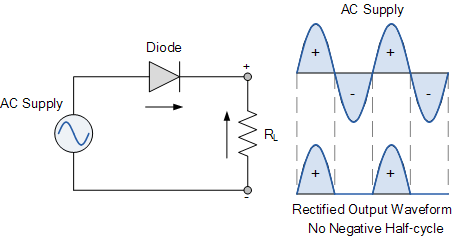
\includegraphics[width=4in]{hwr.png}
\caption{Half Wave Rectifier Circuit (Credit: www.electronics-tutorials.ws)}
\label{fig1}
\end{figure}

If our input signal is an alternating current we can follow this signal at the sinusoidal extremes. So let's start with a positive peak voltage. What will this circuit do?

There would be that peak voltage on the negative side of the diode, thus forward biasing it, so it would open and current would flow.

When there is zero volts, we don't have enough voltage difference to jump electrons across the diode, so current would not flow.

At negative peak voltage, we don't have enough voltage difference to reach the operating point. We would be reversed biased, but probably not by enough to reach the breakdown point, so no current flows.

This causes the voltage on our load resistor to only include the positive portion of our AC signal, but narrowed and dropped slightly by the voltage drop over the diode. So now we have slightly less than half of the power of the AC signal. However this voltage fluctuates quite a bit. If our peak is at 6V and we need at least 5 Volts to charge a battery, for example, for over half of this cycle there isn't a high enough voltage to charge said battery.

Most circuits are designed to work with a specific voltage and dropping too far below or above it can cause the circuit to not work. Many circuits are also hindered and perform at a lower quality when the incoming power is noisy or fluctuates too much. We can add a capacitor in parallel with our load to help smooth this signal out. Since components in parallel have the same voltage, the circuit charges up the capacitor to the peak output voltage. Then during the negative cycle, this capacitor discharges into the load, but loses charge and thus voltage as it does so. We'll come back to this idea later.

Now let's bring in the rest of it and talk about the Full Wave Rectifier. We can see this schematic below.

\begin{figure}[ht]
	\centering
	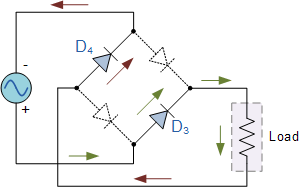
\includegraphics[width=4in]{fwr.png}
	\caption{Full Wave Rectifier Diagram (Credit: www.electronics-tutorials.ws)}
	\label{fig1}
\end{figure}

In the picture above you can see that we have our positive signal going down from the source and negative going up. This opens up $D_{3}$ and $D_{4}$ allowing current to flow through the load and back to the source.
When the AC source flips we'll find the opposite is true. $D_{1}$ and $D_{2}$ open with the others closed, allowing current to still flow positively through the load and back to the source. A simulated output graph can be see below.

\begin{figure}[ht]
	\centering
	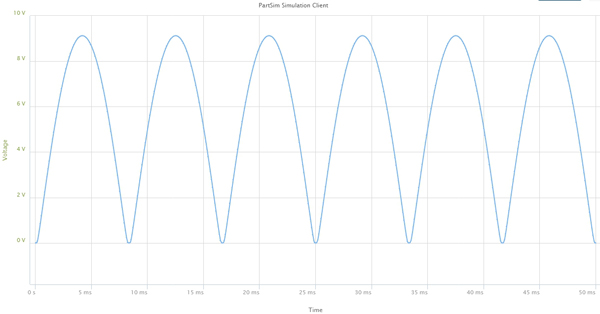
\includegraphics[width=4in]{waveform-1.jpg}
	\caption{Full Wave Rectifier Output (Credit: www.electronics-tutorials.ws)}
	\label{fig1}
\end{figure}

Now we do have the full cycle made positive, which makes this circuit about twice as efficient as the half wave counterpart, but again we see the fluctuating voltage.
Now is the time we can add a capacitor in series with the load to smooth this signal out. It takes time for the capacitor to charge and to discharge, though, and this peak to peak oscillation is known as a ripple voltage. Below you can see the signal somewhat smoothed out with the ripple voltage present.

\begin{figure}[ht]
	\centering
	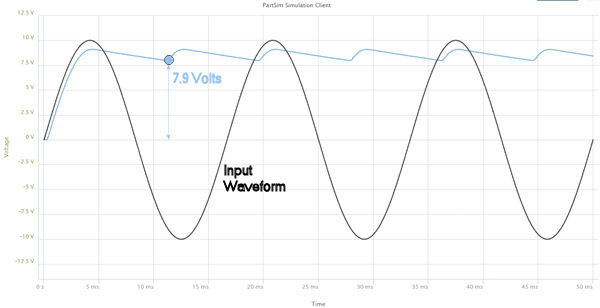
\includegraphics[width=4in]{smoothcap.jpg}
	\caption{Full Wave Rectifier Output Smoothed (Credit: www.electronics-tutorials.ws)}
	\label{fig1}
\end{figure}

It is worth noting that this ripple voltage is based on the time it takes for the capacitor to charge and discharge. These are also dependent on the current of both the source and the load, but it's much easier for us to change the capacitor out for one of a different size. A smaller capacitor, discharging much faster, will increase the size of this ripple voltage, but a larger capacitor will shrink it by staying charged long enough for the next cycle to come and charge it back up. However, these larger capacitors do take longer to charge up in the first place. A large enough capacitor may not be able to fully charge on the first half cycle, and even take multiple cycles to reach the full output voltage, but in return we can smooth this signal out to the point that the ripple voltage becomes negligible and difficult to measure.

\section{Analysis}
Our data showed us the rectification of our signal rather tangibly. It also showed us the "noise" of this signal and why/how we smooth that out. This circuit took us through the steps of power conversions and the efficiencies of it step by step. A Full Wave Rectifier is more practically efficient that its half wave counterpart, and properly smoothed it's even more so.

%\begin{thebibliography}{99}
% The numeral (here 99) in curly braces is nominally the number of entries in
% the bibliography. It's supposed to affect the amount of space around the
% numerical labels, so only the number of digits should matter--and even that
% seems to make no discernible difference.
%Not Requested
%\end{thebibliography}

\end{document}
